\chapter{\textbf{Исследовательский раздел}}

В данном разделе проведено описание экспериментов и их результатов.

\section{Оптимизация параметров модели}

Необходимо оптимизировать параметры, то есть найти такие веса для каждого класса и классификатора (суммарно 22), при которых результаты будут наилучшими.

\section{Метрика для оценки работы классификатора}

В качестве метрик правильности классификации были выбраны точность (precision) и полнота (recall). 

Точность в пределах класса -- это доля фотографий, действительно принадлежащих данному классу документа, относительно всех фотографий, причисленных классификатором к этому классу. 

Полнота системы -- отношение числа найденных классификатором документов, принадлежащих этому классу, к числу всех фотографий этого класса в тестовой коллекции.

\begin{itemize}
\item TP -- истинно-положительное решение.
\item TN -- истинно-отрицательное решение.
\item FP -- ложно-положительное решение.
\item FN -- ложно-отрицательное решение.
\end{itemize}

В таблице \ref{table:metrics} наглядно представлена данная оценка.

\begin{table}[H]
\caption{Оценка качества работы классификатора. }
\begin{tabular}{|l|l|l|l|}
\hline
\multicolumn{2}{|l|}{\multirow{2}{*}{Класс ci}} & \multicolumn{2}{l|}{Экспертная оценка} \\ \cline{3-4} 
\multicolumn{2}{|l|}{} & Положительная      & Отрицательная     \\ \hline
\multirow{2}{*}{Оценка системы} & Положительная & TP & FP \\ \cline{2-4} 
 & Отрицательная & FN & TN \\ \hline
\end{tabular}
\label{table:metrics}
\end{table}

Точность определяется по формуле \ref{eq:prec}.
\begin{equation}
	\centering
	p = \frac{TP}{TP+FP}
	\label{eq:prec}
\end{equation}

Полнота определяется по формуле \ref{eq:rec}.
\begin{equation}
	\centering
	r = \frac{TP}{TP+FN}
	\label{eq:rec}
\end{equation}

Тогда $F_1$-мера, характеризующая точность классификации для одного жанра равна \ref{eq:f1}.
\begin{equation}
	\centering
	F_1=2\frac{p\cdot r}{p + r}
	\label{eq:f1}
\end{equation}

Эффективность классификации для всей выборки рассчитывается как среднее арифметическое $F_1$-мер по всем классам документов.

\section{Процесс оптимизации}

Как было сказано выше оптимизация проводится методом Пауэлла \cite{paul}.

Этот метод предназначен для минимизации квадратичных функций, основывается на их свойстве: любая прямая, проходящая через точку минимума функции, пересекает под равными углами касательные к поверхностям равного уровня функции в точках пересечения. 

Суть метода заключается в следующем. Выбирается начальная точку$x [0]$и выполняется одномерный поиск в любом направлении, в результате чего появится точка$x[1]$. Затем выбирается точка $x[2]$, не лежащую на прямой $x[0];x[1]$, и выполняется одномерный поиск вдоль прямой, параллельной $x[0]; x[1]$. Полученная точка $x[3]$ и точка $x[1]$ определяют направление $x[1];x[3]$ одномерного поиска, приводящего к точке минимума. В случае квадратичной функции n-переменных, оптимальное значение находитя за n итераций. В этом случае поиск минимума осуществляется во взаимно сопряженных направлениях. В случае неквадратичной целевой функции направления поиска сопряжены относительно с матрицы Гессе.

Для исследования на экстремум была взята функция от всех 22 параметров модели, возвращающая суммарную ошибку на обучающей выборке. Ошибка вычислялась как 1 минус средняя F1-мера.

Тогда результирующие веса для разных типов документов.
\begin{itemize}
\item Для классификатора по визуальным признакам:

[0.09, 0.185, 1, 1.1, 1.025, 0.1, 0.188, 1.1, 1.075, 0.138, 1.025]

\item Для классификатора по текстовым признакам: 

[1.1, 1.075, 1, 1.026, 1.1, 1.1, 1.125, 1.05, 0.8, 1.1, 1.125]
\end{itemize}

\section{Оценка эффективности разработанного метода}

Выше делалось предположение, что визы похожи друг на друга визуально, но текстовая информация в них различна. Приведем матрицы ошибок для текстового \ref{img:textclass} и визуального \ref{img:visclass} классификаторов.

\begin{figure}[H]
	\centering
	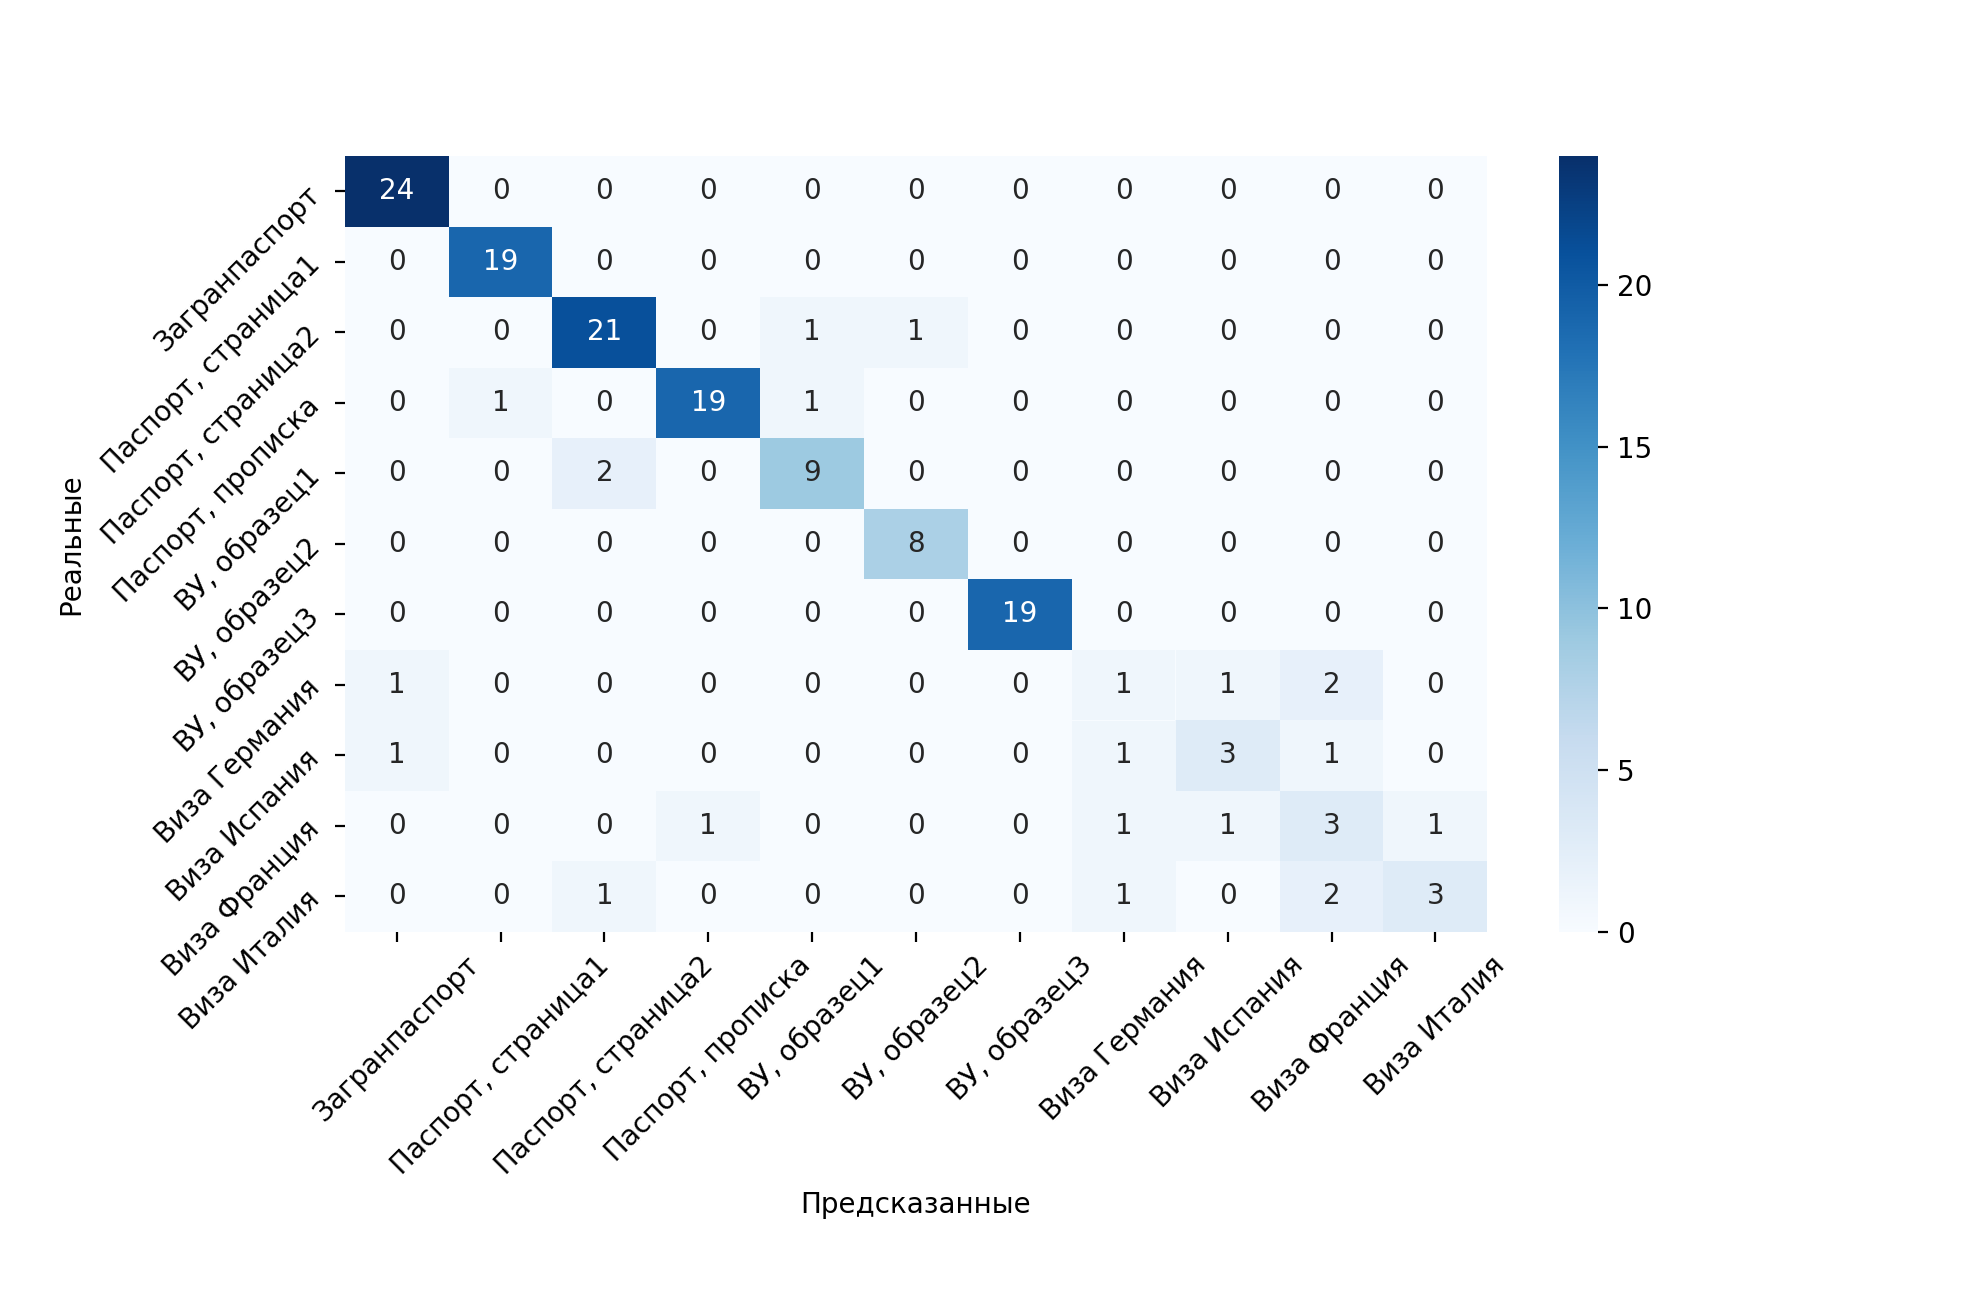
\includegraphics[scale=0.8]{textclass}
	\caption{Матрица ошибок для текстового классификатора. }
	\label{img:textclass}
\end{figure}

\begin{figure}[H]
	\centering
	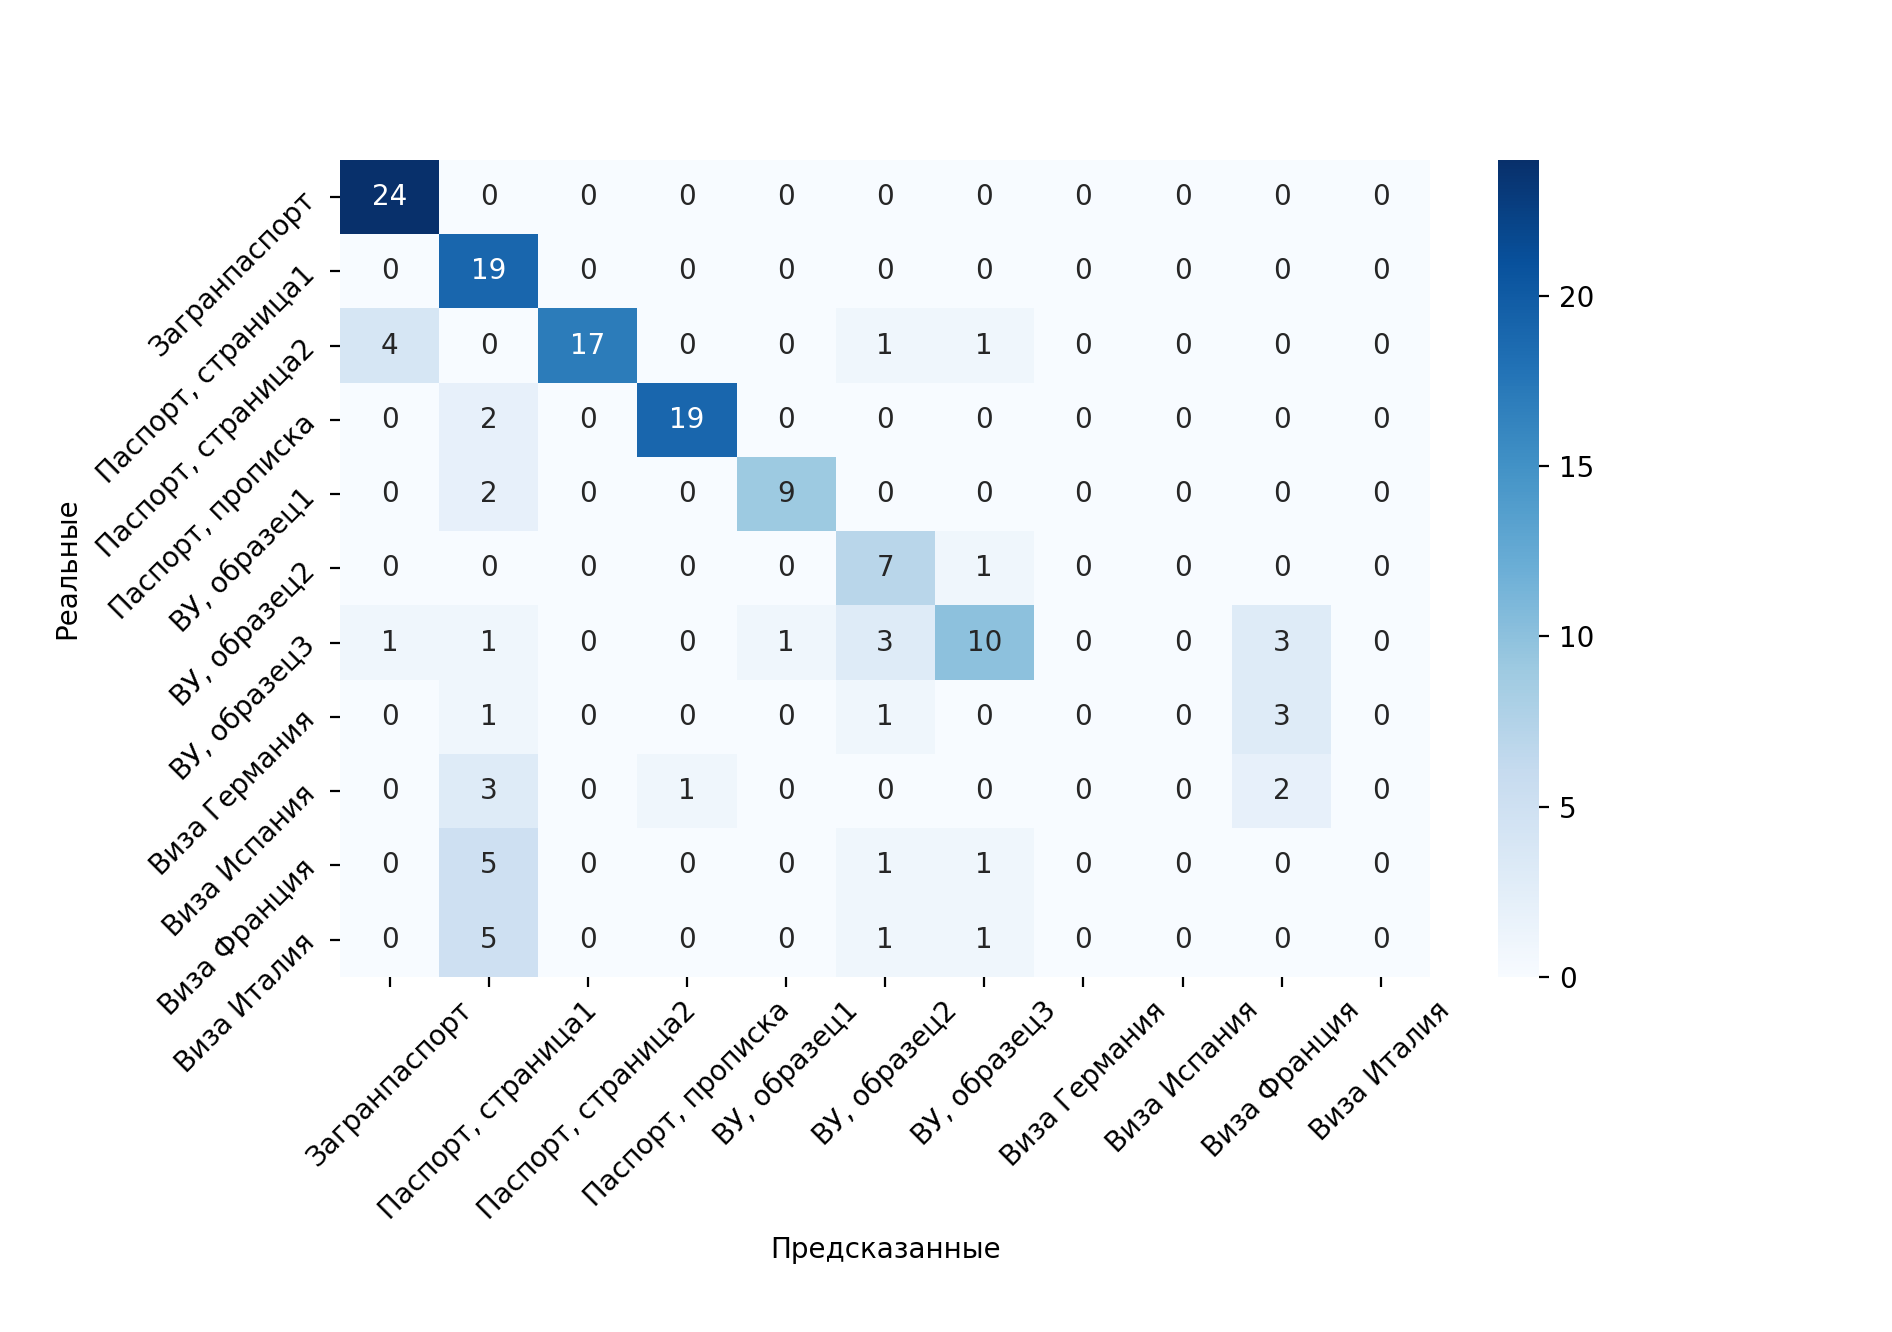
\includegraphics[scale=0.8]{visclass}
	\caption{Матрица ошибок для визуального классификатора. }
	\label{img:visclass}
\end{figure}

Как видно из картинок, визуальный классификатор не справляется с изображениями виз, в основном он их классифицирует, ка первую страницу паспорта.

А вот текстовый классификатор справился лучше, да он часто путается в типе виз (так как очень много текста там повторяется), но он мало ошибается именно с определением, что выбранный документ виза.

Далее представлено сравнение результатов работы объединенного классификатора, текстового и визуального \ref{img:graph}. С помощью метрики $F_1$.

\begin{figure}[H]
	\centering
	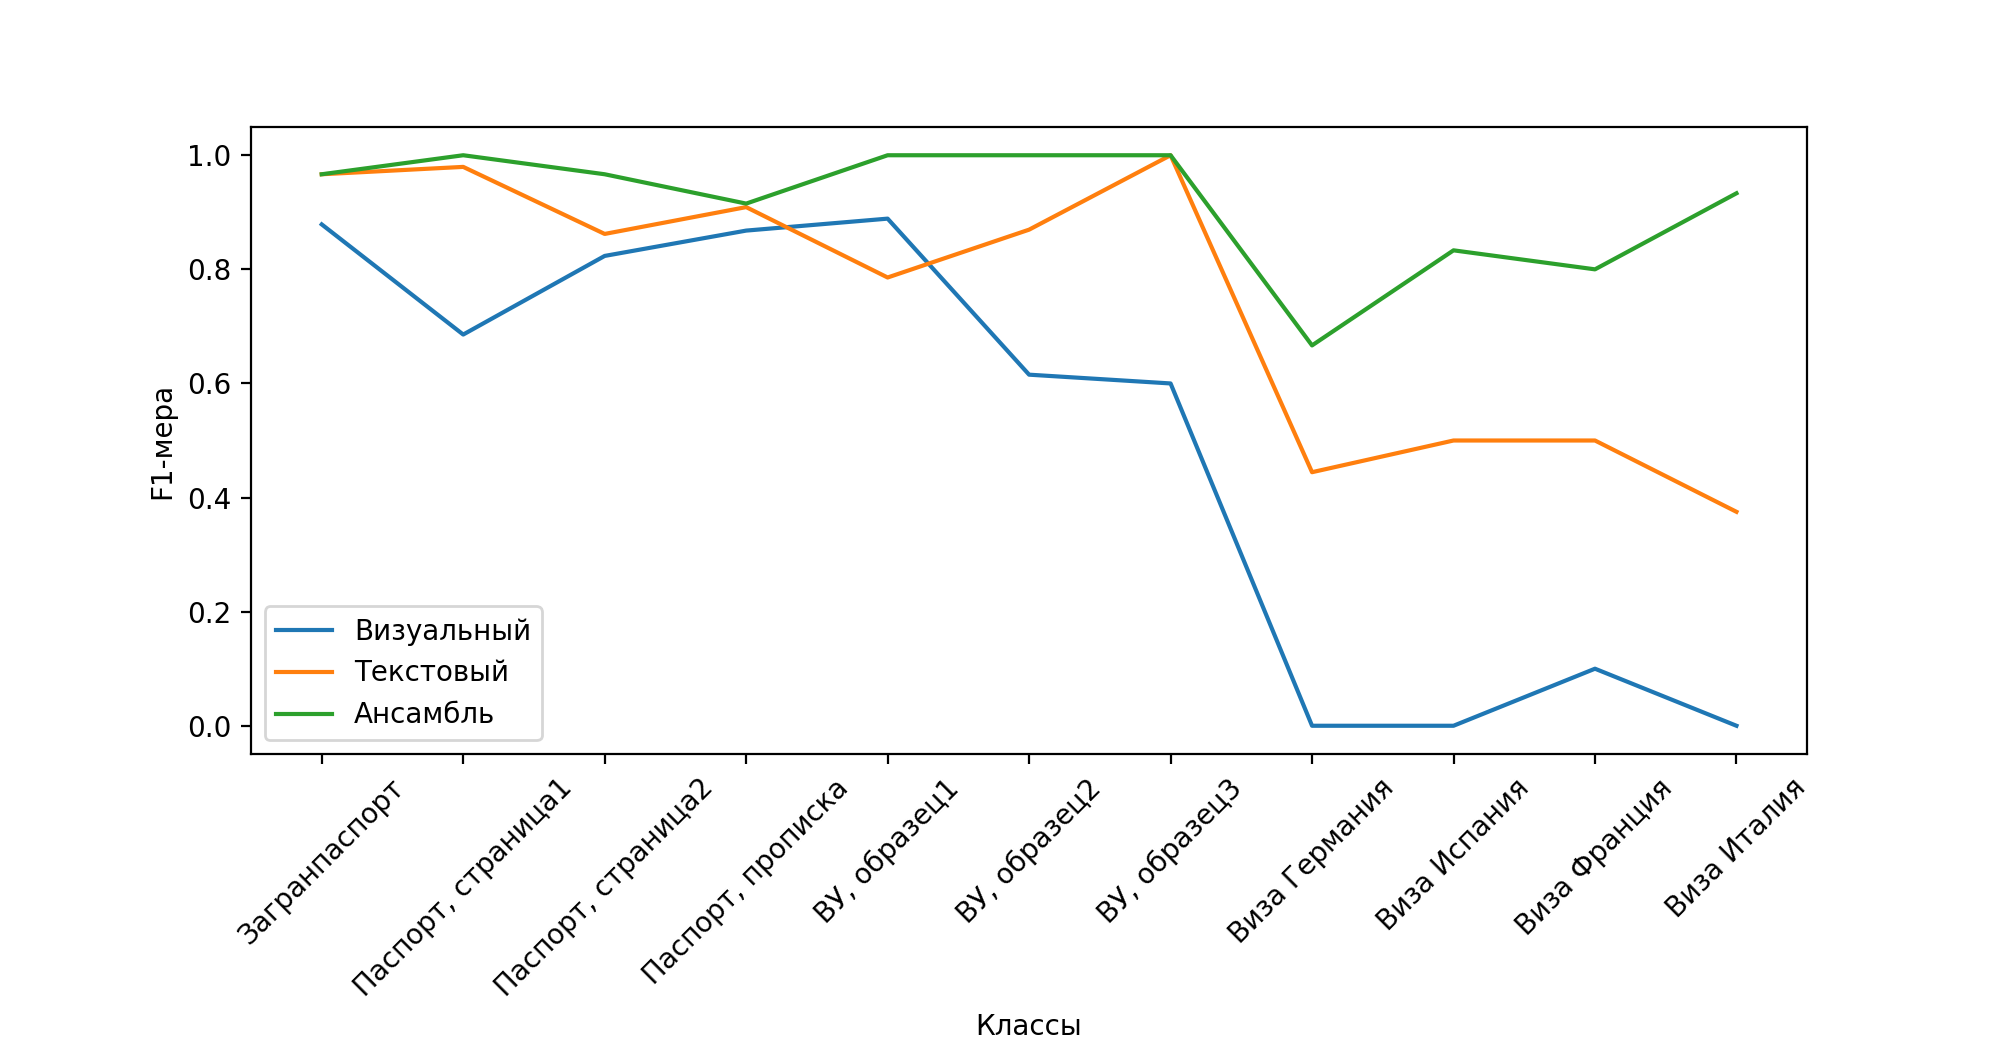
\includegraphics[scale=0.73]{graph}
	\caption{Сравнение F1-мер для классификаторов. }
	\label{img:graph}
\end{figure}

\section{Вывод}

Полученные оптимальные весовые коэффициенты были применены на практике. Из графика видно, что F1-мера ансамбля классификаторов по всем классам превосходит либо равна F1-мерам визуального и текстового классификаторов, что свидетельствует об успешном улучшении метода.
